\chapter{RELATO DO EXPERIMENTO}

\begin{figure}[H]
	\centering
	\caption{Engenheiro Eletricista}
	\label{fig:engenheiroeletricista}
	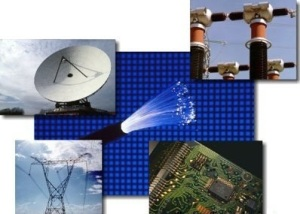
\includegraphics[width=0.7\linewidth]{data/figures/EngenheiroEletricista}
	\fonte{\citeonline{ref:ufersa-caraubas}}
\end{figure}

A Engenharia Elétrica está presente na fabricação de praticamente todo produto manufaturado e daqueles que envolvem alta tecnologia, como satélites, aeronaves e produtos utilizados na automação industrial. Na verdade, esta engenharia se subdivide em várias áreas, como Eletrotécnica, Controle e Automação, Eletrônica, Microeletrônica e Telecomunicações.

O campo de atuação de um engenheiro eletricista é bastante amplo. Ele pode desenvolver atividades nas áreas de sistemas de geração, transmissão e distribuição de energia elétrica, controle e automação, instrumentação, sistemas eletrônicos analógicos e digitais, e projeto de circuitos integrados. Pode atuar no ramo das telecomunicações, em telefonia, antenas e propagação, na construção civil, na manutenção industrial, em informática, só para citar algumas possibilidades.

O profissional com formação em Engenharia Elétrica pode atuar não apenas em instituições privadas, mas também em órgãos governamentais, como agências reguladoras, secretarias, ministérios e autarquias em geral.
O mercado de trabalho está bem aquecido. As maiores oportunidades estão nas grandes e médias empresas multinacionais e em algumas nacionais. São crescentes também as possibilidades nas pequenas empresas nacionais que estão se modernizando para competir no mundo globalizado.

O engenheiro eletricista pode ainda seguir a carreira científica, atuando em centros de pesquisa e em universidades. Como em qualquer outra área de atuação, a preocupação com o ser humano e o meio ambiente é algo indispensável ao engenheiro formado atualmente.